\chapter{Tradução de ROBO para CSP}
A Seção 3.1 descreve como foi realizado o processo de tradução automático de ROBO para CSP através do framework Spoofax. Desde a fase inicial da definição da gramática até a geração de código.

\section{Processo de Tradução Automática}

\subsection{Ferramentas e Ambiente de Programação}
O desenvolvimento de um compilador exige uma preparação bem elaborada de todo um ambiente de programação. No caso deste trabalho, foi necessário o uso do ambiente de programação Eclipse juntamente com um plugin do Spoofax. O qual foi essencial para o desenvolvimento da abordagem de tradução automática. O plugin tem todas as depedências para a geração de Árvore de Análise Sintática e tranformação de código.

\section{Definição da Linguagem ROBO com Spoofax}
Nesta Seção veremos como ocorrreu todo o processo de definição da linguagem ROBO usando o framework Spoofax, o que inclui a definição da sintaxe e transformação da linguagem, resultando em código CSP.
\subsection{Definição da Sintaxe}
Essa é a etapa inicial para a construção do compilador, na qual devemos primeiro definir todos os aspectos da sintaxe da linguagem de programação utilizada no ambiente RoboMind. Ou seja, essa etapa deverá ser capaz de considerar os programas escritos na linguagem ROBO e dizer se eles estão sintaticamente corretos, como produto disso é gerado uma Árvore Sintática Abstrata (\textit{Abstract Syntax Tree - AST}, em inglês).

É importante saber que linguagem ROBO possui algumas características que difere da linguagens de programação, uma vez que se trata de uma DSL, com um objetivo bem definido. Abaixo estão listados algumas das principais características de ROBO:

\begin{itemize}
    \item Funções booleanas predefinidas para detecção de obstáculos ou objetos ao redor do robô, por exemplo \textit{frontIsObstacle}, para verificar se há obstáculo na frente do robô ou \textit{frontIsClear}, para verificar se a frente do robô está livre de quaisquer objetos.
    \item Funções predefinidas para a movimentação do robô, como por exemplo \textit{forward(n)}, para movimentar para frente ou \textit{backward(n)}, para movimentar para trás.
    \item Variáveis globais.
    \item Procedimentos parametrizados e não parametrizados.
    \item Estruturas condicionais e de repetição, assim como na maioria das linguagens de programação.
    \item Expressões aritméticas com valores inteiros.
\end{itemize}

Para exemplificar todo o processo de compilação, definimos um exemplo de programa em ROBO que resolve um problema específico. O problema definido foi "Contando Caixas", proposto por RoboLab-FURB\ref{add-ref} e adaptamos para esta pesquisa. O objetivo desse problema é propor uma solução para simular a contagem de caixas, sendo que a quantidade o usuário deverá indicar o lado para o qual o robô deverá contar, sendo esquerda ou direita. Na Figura \ref{fig:map} é mostrado um mapa utilizado para a simulação do problema em questão. Nela é possível ver o robô e 5 caixas, duas na linha superior e três na linha inferior.

\begin{figure}[h]
\centering
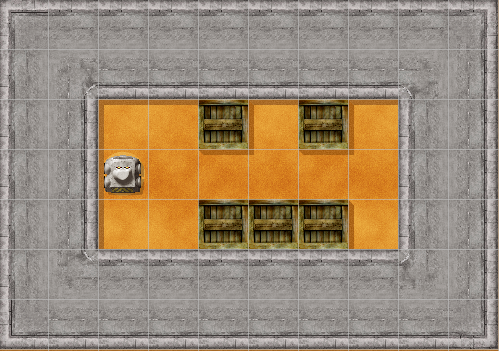
\includegraphics[height=7cm]{figuras/map.png}
\caption{Exemplo de Mapa usado no RoboMind}
\label{fig:map}
\end{figure}

Na Figura \ref{fig:roboprogram} está disposto o código de um programa que resolve o problema da contagem de caixas. Esse programa possui duas variáveis globais: (a) \textit{countBoxes}, que é responsável por amazenar a quantidade de caixas; e (b) \textit{lookLine}, que é para indicar qual a linha que o robô deve contar as caixas (esquerda ou direita). Também há um procedimento parametrizado chamado \textit{countLine()}, este possui um único parâmetro denominado \textit{side}, o qual indicará o lado que o robô irá analisar. Se o valor passado ao parâmetro for igual a 1, então contará as caixas do lado esquerdo, se for qualquer valor diferente de 1, então contará as caixas do lado direito. O primeiro movimento do robô ocorre através do comando \textit{right} (indicado na linha 16), o qual altera sua orientação em 90 graus à direita. O próximo passo é a execução de um laço pelo comando \textit{repeatWhile}, a repetição ocorre enquanto não houver quaisquer objetos ou paredes na célula à frente do robô. Esse laço é responsável por chamar o procedimento \textit{countLine()} passando o valor da variável \textit{lookLine}, que neste exemplo tem valor 1, ou seja, contará as caixas da linha esquerda, seguindo de um \textit{forward} que move o robô para frente em uma unidade a cada execução do laço. Ao sair dessa estrutura de repetição, o procedimento será executado mais uma vez, com o objetivo de verificar possíveis caixas na última posição do robô e por fim a quantidade de caixas é exibida por meio do comando \textit{show} exibindo o valor armazenado na variável \textit{countBoxes} contendo a quantidade de caixas na linha de interesse. Este exemplo servirá para toda as etapas, desde a geração de uma AST, após a execução do parser, até a geração de código CSP, após a transformação da árvore.

\begin{figure}[h]
\lstinputlisting{codes/program1.rob}
\caption{Programa escrito em ROBO}
\label{fig:roboprogram}
\end{figure}

O trabalho descrito em XX, como já mencionado, propõe um compilador que contempla a tradução de programas ROBO sem variáveis e procedimentos. No entanto, a gramática definida resulta uma AST é um formato  Program(Sequence, Sequence) similar a uma tupla o que impossibilitava o uso de funções do framework Spoofax que facilitassem a transformação da árvore, como por exemplo, aplicação de filtros e recolhimento de \textit{Terms} específicos. Sabendo disso, para facilitar o trabalho em cima da árvore, foi necessário reconstruir partes da gramática de modo que a AST gerada tivesse um formato de lista, assim tornando possível o uso das funções nativas do Spoofax. Na Figura \ref{fig:gramatica_antes} tem um trecho da gramática definida no trabalho citado.

\begin{figure}[h]
\lstinputlisting[language=Java]{codes/gramatica_antes.sdf3}
\caption{Gramática escrita em forma de sequência}
\label{fig:gramatica_antes}
\end{figure}

Já na Figura \ref{fig:gramatica} a gramática foi totalmente reescrita, antes o que era \textit{Sequence} tornou-se \textit{Statement} seguido pelo operador * de concatenação. Dessa forma, ao invés do programa iniciar com uma \textit{Sequence}, a qual também chamava uma \textit{Sequence} precedida de uma \textit{Instr}. Além dessa mudança, foi adicionado o termo \textit{Declaration} (linha 6) que possui três tipos: \textit{Variable}, \textit{Procedure} e \textit{ProcParam} (linhas 8, 9 e 12, respectivamente).

\begin{figure}[h]
\lstinputlisting[language=Java]{codes/gramatica.sdf3}
\caption{Gramática escrita em forma de lista}
\label{fig:gramatica}
\end{figure}

\subsection{Transformação com Stratego}

